\documentclass{article}

\usepackage{amsmath}
\usepackage{amssymb}
\usepackage[spanish]{babel}
\usepackage{cancel}
\usepackage[margin=1.5in]{geometry}
\usepackage{graphicx}
\usepackage[utf8]{inputenc}
\usepackage{tcolorbox}

\renewcommand{\Bbb}{\mathbb}

\tcbuselibrary{theorems}

\begin{document} 

\section{T1}

\subsection{El espacio vectorial $\Bbb R^n$}

El objetivo de la materia es adaptar los conceptos de Análisis I (derivadas, integrales, Taylor ...) al espacio n-dimensional, $\mathbb{R}^n$.

\begin{equation}
x \in \Bbb R^n \Longleftrightarrow x = (x_1, x_2, x_3, ..., x_n)
\end{equation}

Se dice que $x$ es un vector o punto de $\Bbb R^n$, compuesto por $n$ números reales. No se distingue entre vector y punto, salvo que sea necesario.

$\Bbb R^n$ se estructura en espacio vectorial definiendo las siguientes operaciones:

\begin{subequations}
\begin{align}
\forall x, y \in \Bbb R^n, & z = x + y \Longleftrightarrow z_i = x_i + y_i, \forall i \in [1, n] & \text{SUMA VECTORIAL}\\
\forall \alpha \in \Bbb R, & x \in \Bbb R^n, z = \alpha x \Longleftrightarrow z_i = \alpha x_i \forall i \in [1, n] & \text{PRODUCTO POR ESCALAR}
\end{align}
\end{subequations}

Con estas definiciones, puede probarse que $\Bbb R^n$ es cerrado para la suma vectorial y producto por un escalar, considerando el vector nulo (todos ceros), $\overline{0}$, como el neutro para la suma, y el número real 1 como el neutro del producto por escalar.

Adicionalmente, $\Bbb R^n$ pasa a ser un \textbf{espacio vectorial euclídeo} si se le agrega un \textbf{producto escalar}:

\begin{equation}
\forall x, y \in \Bbb R^n, \alpha = x \cdot y \Longleftrightarrow \alpha = \sum_{i=1}^{n} x_i y_i = x_1 y_1 + x_2 y_2 + ... + x_n y_n
\end{equation}

Definiendo una \textbf{norma} sobre el producto escalar, $\Bbb R^n$ pasa a ser un espacio vectorial euclídeo y normado. La norma canónica en $\Bbb R^n$ es la raíz cuadrada del producto escalar del vector consigo mismo:

\begin{equation}
\forall x \in \Bbb R^n, \|x\| = \sqrt{x \cdot x} = \sqrt{ \sum_{i=1}^{n} x_i^2 }
\end{equation}

Un \textbf{versor} es un vector de norma 1. Para "normalizar" cualquier vector, se lo divide por su norma:

\begin{equation}
\forall x \in \Bbb R^n, \left\| \frac{x}{\|x\|} \right\| = 1
\end{equation}

\subsection{Ángulo entre dos vectores - Proyección}

Si $x, y \neq \overline{0}$, el ángulo entre x e y, $\alpha(x,y)$, satisface la siguiente igualdad:

\begin{equation}
\cos (\alpha(x, y)) = \frac{x \cdot y}{ \|x\| \|y\| }
\end{equation}

\begin{figure}[t]
\caption{Proyección del vector x sobre el vector y}
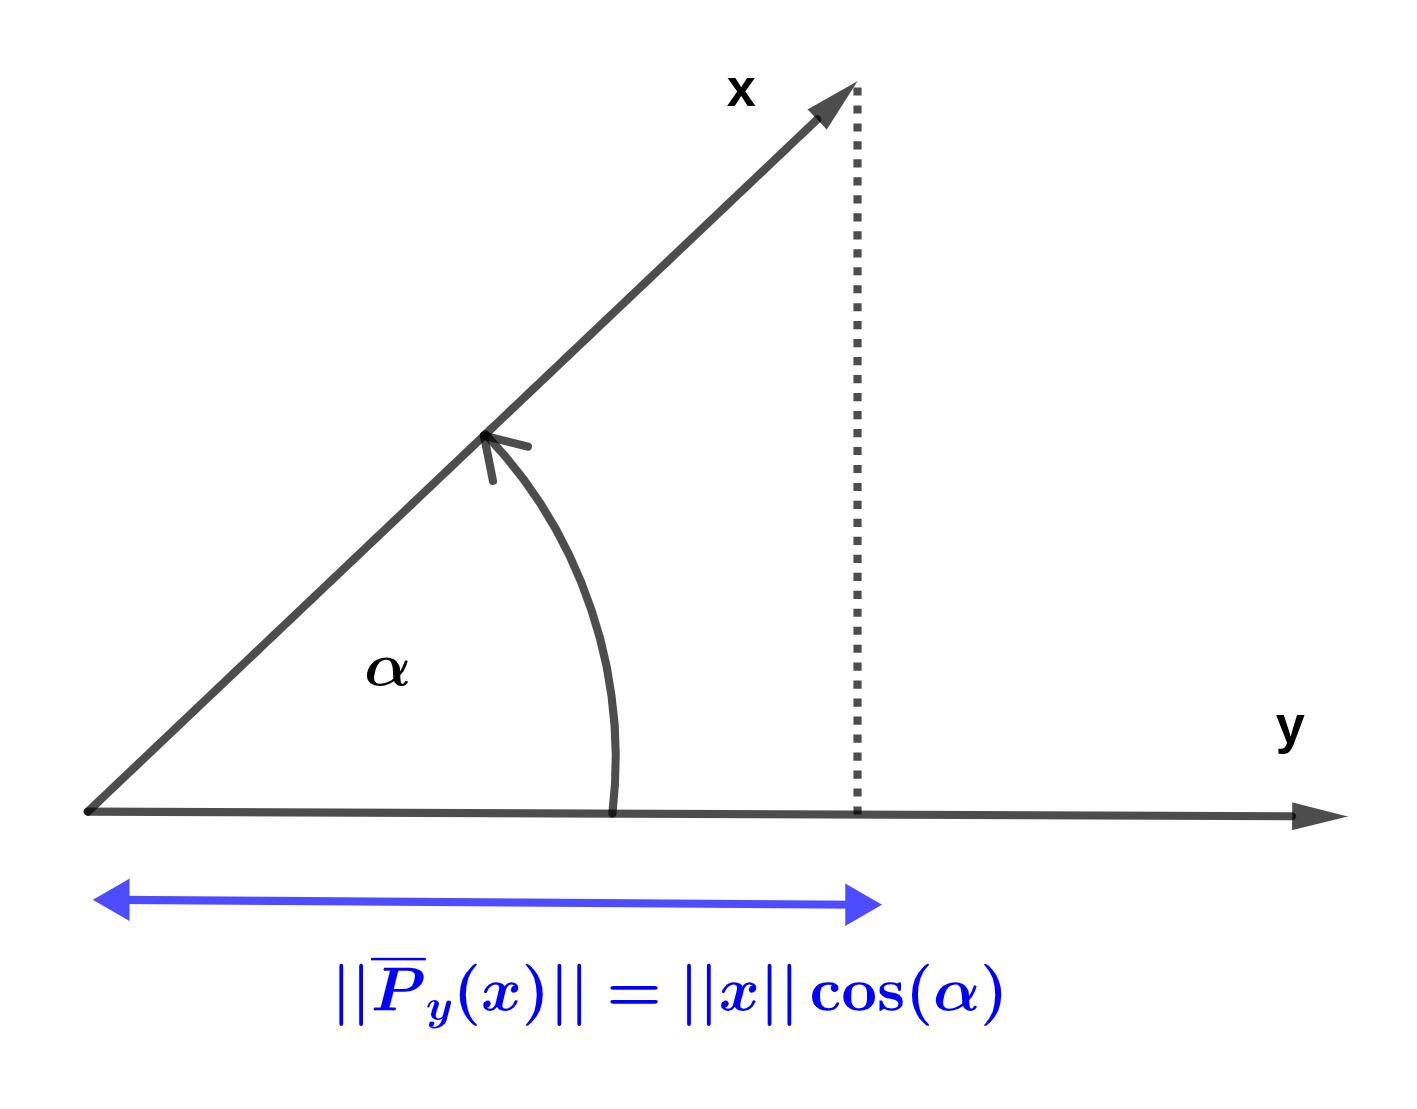
\includegraphics[scale=1]{img/teo_fig001_proyeccion.png} 
\centering
\label{fig:proyeccion}
\end{figure}

Aplicando la igualdad del ángulo entre vectores, y considerando el versor $\breve{y} = \frac{y}{\|y\|}$, resulta:

\begin{equation}
x \cdot y = \|x\| \|y\| \cos(\alpha) \Longrightarrow x \cdot \breve{y} = \|x\| \underbrace{ \cancel{ \| \breve{y} \| } }_{\text{Norma 1}} \cos(\alpha) = \|x\| \cos(\alpha)
\end{equation}

Geométricamente, como se observa en la figura ~\ref{fig:proyeccion}, la proyección de x sobre y se obtiene como el siguiente vector:

\begin{equation}
\overline{P}_{y}(x) =  \underbrace{ \|x\| \cos(\alpha) }_{\text{Escalar}}  \underbrace{ \breve{y} }_{\text{Versor}}
\end{equation}

\begin{equation}
\tcboxmath[colback=orange!25!white,colframe=orange, title=Proyección de x sobre y]
{ \overline{P}_{y}(x) = (x \cdot \breve{y}) \breve{y} }
\end{equation}

\begin{subequations}
\begin{align}
\overline{P}_{y}(x) = \overline{0} & \Longleftrightarrow x \perp y \Longleftrightarrow \cos \alpha = 0 \\
\overline{P}_{y}(x) = x & \Longleftrightarrow x = \alpha y, \alpha > 0
\end{align}
\end{subequations}

\subsection{Distancia entre dos puntos}

$\forall x, y \in \Bbb R^n$, se define la distancia entre x e y como:

\begin{equation}
d(x,y) = \| x - y \| = \| y - x \|
\end{equation}

\subsection{Producto vectorial}

Sólo para $\Bbb R^3$, se define el \textbf{producto vectorial} como:

\begin{equation}
\forall x, y \in \Bbb R^3: x \otimes y = \begin{vmatrix}
    \breve{i} & \breve{j} & \breve{k} \\
    x_1 & x_2 & x_3 \\ 
    y_1 & y_2 & y_3
  \end{vmatrix} =
\left(
  \begin{vmatrix} x_2 & x_3 \\ y_2 & y_3 \end{vmatrix},
  -\begin{vmatrix} x_1 & x_3 \\ y_1 & y_3 \end{vmatrix},
  \begin{vmatrix} x_1 & x_2 \\ y_1 & y_2 \end{vmatrix}
\right)
\end{equation}

Propiedades:

\begin{subequations}
\begin{align}
x \otimes y & \perp x \\
x \otimes y & \perp y \\
x \otimes y & = -y \otimes x \\
\| x \otimes y \| & = \|x\| \|y\| \sin(\alpha(x,y)) = \text{Área del paralelogramo determinado por x e y} \\
x \otimes y & = \overline{0} \Longleftrightarrow \{x, y\} \text{ es linealmente dependiente} \Longleftrightarrow x \parallel y
\end{align}
\end{subequations}

\subsection{Clasificación de puntos en un subconjunto de $\Bbb R^n$}

Sea un punto $P_0 \in \Bbb R^n$; se define como \textbf{bola o entorno} de centro $P_0$ y radio $r$ al conjunto de puntos cuya distancia a $P_0$ es menor que $r$. Simbólicamente:

\begin{equation}
B(P_0, r) = \{ x \in \Bbb R^n / \| x - P_0 \| < r \}
\end{equation}

En $\Bbb R$, esto es un intervalo abierto; en $\Bbb R^2$, el interior de un círculo; en $\Bbb R^3$, el interior de una esfera. Para dimensiones mayores, no hay tal representación geométrica, pero la definición se mantiene.

Si se excluye al centro $P_0$, se habla de una bola o entorno \textbf{reducido}:

\begin{equation}
B^*(P_0, r) = B(P_0, r) - \{ P_0 \}
\end{equation}

Considérese a continuación un subconjunto $A \subseteq \Bbb R^n$

\subsubsection{Punto interior}

$P_0$ es punto interior de $A \Longleftrightarrow \exists B(P_0, r) \subset A$. Es decir, si existe al menos un entorno centrado en $P_0$ que esté incluido en $A$. En otras palabras, $P_0$ está "rodeado por todas partes" de puntos de $A$.

Por otro lado, se define al \textbf{conjunto interior de} $A$, notado $\mathring{A}$, de la siguiente manera:

\begin{equation}
\mathring{A} = \{ x \in \Bbb R^n / x \text{ es punto interior de } A \}
\end{equation}

\subsubsection{Punto exterior}

$P_0$ es punto exterior de $A \Longleftrightarrow \exists B(P_0, r) \subset A^c$. Es decir, un punto es exterior de $A$ si es interior del complemento de $A$ ($A^c$).

\begin{equation}
Ext(A) = \{ x \in \Bbb R^n / x \text{ es p.e. de A } \}
\end{equation}

\subsubsection{Punto frontera}

$P_0$ es punto frontera de $A \Longleftrightarrow$ toda bola centrada en $P_0$ contiene elementos de $A$ y $A^c$. Simbólicamente:

\begin{equation}
P_0 \text{ es p.f. de } A \Longleftrightarrow \forall B(P_0, r), \left\{
\begin{array}{ll}
B(P_0, r) \cap A \neq \varnothing \\
B(P_0, r) \cap A^c \neq \varnothing
\end{array}
\right.
\end{equation}

La \textbf{frontera} de $A$, $\partial A$, se define como:

\begin{equation}
\partial A = \{ x \in \Bbb R^n / x \text{ es p.f. de A } \}
\end{equation}

Propiedades:

\begin{subequations}
\begin{align}
\mathring{A} \cap \partial A & = \varnothing \\
Ext(A) \cap \partial A & = \varnothing \\
\mathring{A} \cap Ext(A) & = \varnothing \\
\mathring{A} \cup \partial A \cup Ext(A) & = \Bbb R^n \\
\text{Clausura/adherencia de A } = \overline{A} & = A \cup \partial A \\
\text{A es abierto } \Longleftrightarrow A & = \mathring{A} \\
\text{A es cerrado } \Longleftrightarrow A & = \overline{A} \Longleftrightarrow A^c \text{ es abierto } \\
\end{align}
\end{subequations}

\subsubsection{Punto aislado}

$P_0$ es p.a. $\Longleftrightarrow \exists B^*(P_0, r) / B^*(P_0, r) \cap A = \varnothing$.

O sea, hay al menos un entorno reducido centrado en $P_0$ que no contiene otro elemento de $A$ aparte de $P_0$.

\subsubsection{Punto de acumulación}

$P_0$ es p. de ac. $\Longleftrightarrow \forall B^*(P_0, r), B^*(P_0, r) \cap A \neq \varnothing$.
Vale decir, en todo entorno reducido de $P_0$ hay elementos de $A$. El conjunto derivado de $A$, denotado $A'$, se define como el conjunto de todos los puntos de acumulación de $A: A' = \{ x \in \Bbb R^n / x \text{ x es p. de ac. de A} \}$

\section{T2 - Funciones}

\begin{subequations}
\begin{align}
f: A \rightarrow B \\
A = \text{dominio de f} \\
B = \text{codominio/imagen de f} = Im(f) \\
\text{Gráfico de f } = G(f) = \{ (x, f(x)) \text{ con x } \in A \}
\end{align}
\end{subequations}

Si $A \subset \Bbb R^n$ y $B \subset \Bbb R^m$, entonces $G(f) \subset \Bbb R^(n+m)$.

$x$ es el argumento de $f$, y $f(x)$ es la imagen de $x$ a través de $f$.

\subsection{Preimagen}

\begin{equation}
f^{-1}(H) = \{ x \in A / f(x) \in H \}
\end{equation}

$f^{-1}(H)$ NO es la inversa de $f$; esto es notación.

En palabras, la preimagen del conjunto $H$ consiste de los elementos del dominio cuya imagen a través de $f$ pertenece a $H$.

\begin{equation}
H \cap Im(f) = \varnothing \Longrightarrow f^{-1}(H) = \varnothing
\end{equation}

\subsection{Tipos de funciones}

i) Funciones escalares: $A \subset \Bbb R$, $B \subset \Bbb R \Longrightarrow f: \Bbb R \rightarrow \Bbb R$

ii) Campos escalares: $A \subset \Bbb R^n, B \subset \Bbb R \Longrightarrow \overline{f}: \Bbb R^n \rightarrow \Bbb R$

iii) Funciones vectoriales (curvas): $A \subset \Bbb R, B \subset \Bbb R^n \Longrightarrow \overline{f}: \Bbb R \rightarrow \Bbb R^n$

iv) Campos vectoriales: $A \subset \Bbb R^n, B \subset \Bbb R^m \Longrightarrow \overline{f}: \Bbb R^n \rightarrow \Bbb R^m$

\subsection{Conjuntos de nivel}

Partiendo de la definición de preimagen, si $H$ tiene un único elemento $u$, se llama conjunto de nivel $u$ de $f$ a:

\begin{equation}
C_u(f) = \{ x \in A / f(x) = u, u \in B \}
\end{equation}

$u$ puede ser un vector o escalar.

\subsection{Conjunto conexo}

$A \subset \Bbb R^n$ es conexo $\Longleftrightarrow \nexists \text{ dos conjuntos } A_1 y A_2 / A = A_1 \cup A_2$, con $\overline{A_1} \cap A_2 = \varnothing \wedge A_1 \cap \overline{A_2} = \varnothing$.

O sea, no se puede "partir en dos" a $A$.

Construyendo sobre esta definición, $A \subset \Bbb R^n$ es \underline{arco-conexo} si cualquier par de puntos de $A$ puede ser unido a través de una curva continua. Simbólicamente:

\begin{equation}
A \subset \Bbb R^n \text{ es arco-conexo } \Longleftrightarrow \exists \overline{f}: [a,b] \rightarrow A / \overline{f}(a) = x \wedge \overline{f}(b) = y \forall x,y \in A
\end{equation}

\subsection{Conjunto acotado}

$A \subset \Bbb R^n$ es acotado $\Longleftrightarrow \forall x \in A, \exists M > 0 / \|x\| < M$. Vale decir, todo $A$ puede ser contenido en una bola de radio $M$.

\section{T3 - Límite y continuidad}

Un plano puede verse como la imagen de un campo vectorial. Si $\pi: P_0 + \alpha \overrightarrow{u} + \beta \overrightarrow{v}$ (el plano que pasa por $P_0$ y es generado por $\overrightarrow{u}$ y $\overrightarrow{v}$, entonces puede definirse el siguiente campo vectorial:

\begin{equation}
\overline{f}: \Bbb R^2 \rightarrow \Bbb R^3 / \overline{f}(\alpha, \beta) = (x, y, z) = P_0 + \alpha \overrightarrow{u} + \beta \overrightarrow{v}
\end{equation}

Algo análogo puede hacerse con la recta:

\begin{equation}
L = P_0 + t \overrightarrow{u} \longrightarrow \overline{f}: \Bbb R \rightarrow \Bbb R^3 / \overline{f}(t) = P_0 + t \overrightarrow{u}
\end{equation}

Viendo esto físicamente, $t$ puede ser el tiempo, y $\overline{f}$ la trayectoria de un Movimiento Rectilíneo Uniforme.

\subsection{Límite y continuidad}

Generalizando, sea $f: A \rightarrow B$, con $A, B \in \Bbb R^n$

Sea $P_0$ un punto de acumulación de $A$. Se dice que $L \in B$ es el límite de $f$ cuando $P$ tiende a $P_0$ si:

\begin{equation}
\lim_{P \rightarrow P_0}f(P) = L \longleftrightarrow \forall E(L, \epsilon) \exists E^*(P_0, \delta) / [f(E^*(P_0, \delta) \cap A)] \subset E(L, \epsilon)
\end{equation}

\begin{figure}[t]
\caption{Límite}
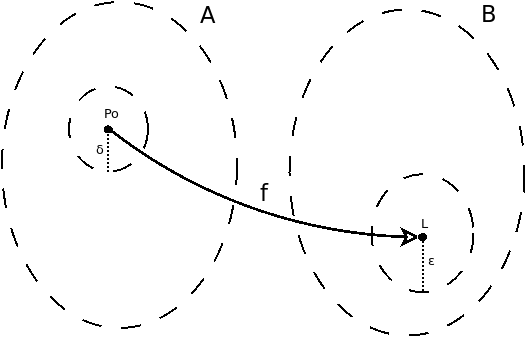
\includegraphics[scale=0.75]{img/teo_fig002_limite.png} 
\centering
\label{fig:limite}
\end{figure}

Como se observa en la figura ~\ref{fig:limite}, el concepto es que, si existe el límite, no importa cuánto se acerque a cero el infinitésimo $\delta$ en el dominio $A$; siempre habrá un entorno centrado en $L$, de radio infinitésimo $\epsilon$, que contenga las imágenes del entorno dominio.

\subsubsection{Aproximación con curva}

\begin{figure}[t]
\caption{Límite}
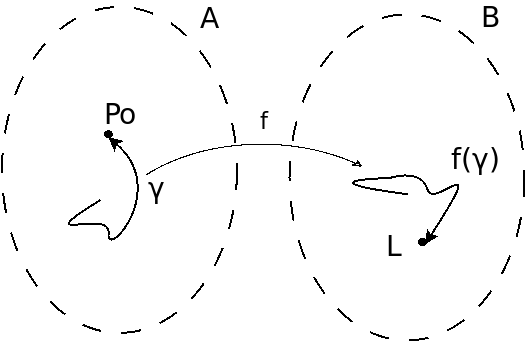
\includegraphics[scale=0.75]{img/teo_fig003_limite_curva.png} 
\centering
\label{fig:limite_curva}
\end{figure}

Lo que pretende mostrar la figura ~\ref{fig:limite_curva} es que, siempre asumiendo que existe el límite, si la aproximación en el dominio se hace con una curva $\gamma$ en lugar de un entorno, la imagen de dicha curva, $f(\gamma)$, convergerá hacia $L$ a medida que $\gamma$ se aproxime a $P_0$. El camino que siga dependerá de cómo transforme f los puntos de $\gamma$.

\subsubsection{Continuidad}

$f$ es continua en $P_0 \longleftrightarrow \displaystyle{\lim_{P \rightarrow P_0}} f(P) = f(P_0)$. En todo otro caso, $f$ es discontinua en $P_0$ de forma \textbf{esencial} si L no existe o es infinito, y de forma \textbf{evitable} si el límite existe, pero $L \neq f(P_0)$ o $\nexists f(P_0)$.

\subsubsection{Unicidad del límite}

Si $L$ existe, es único. Como en Análisis I, esto indica que uno forma de demostrar que un límite no existe, es mostrar que da diferentes valores al calcularlo de diferentes maneras.

\subsubsection{Inexistencia y unicidad}

En funciones de $\Bbb R$ en $\Bbb R$, la existencia e igualdad de los límites laterales garantizaba la existencia del límite, porque sólo había dos direcciones, Sin embargo, en $\Bbb R^n$ hay infinitas formas de aproximarse a un punto; ergo, la igualdad de límites (iterados, radiales, etc) no asegura nada. Sin embargo, si dos difieren, el límite definitivamente no existe.

\subsubsection{Límite de funciones vectoriales}

Para toda función vectorial, el vector límite existe si y sólo si existe el límite para cada uno de los componentes del vector. Por ejemplo:

\begin{equation}
\lim_{t \rightarrow 0} \left( \frac{\sin t}{t}, (1 + t)^\frac{1}{t}, \frac{1-\cos t}{t} \right) = \left( \lim_{t \rightarrow 0} \frac{\sin t}{t}, \lim_{t \rightarrow 0} (1 + t)^\frac{1}{t}, \lim_{t \rightarrow 0} \frac{1-\cos t}{t} \right) = (1, e, 0)
\end{equation}

En este caso, los tres límites existen, y por ende el límite existe. Pero si al menos uno no existiera, dejaría de existir el de la función vectorial.

\subsubsection{Límite de campos escalares}

Ejemplo 1: Sea

\begin{equation}
f(x,y) = x^2 + y
\end{equation}

Es bastante evidente que esta función es continua en todo su dominio; no hay singularidades de ningún tipo. Eso nos permite afirmar, por ejemplo:

\begin{equation}
\lim_{(x,y) \rightarrow (2,1)} f(x,y) = f(2,1) = 5
\end{equation}

Ejemplo 2: Sea

\begin{equation}
f(x,y) = \frac{x^2 - y^2}{x^2 + y^2} \Rightarrow \lim_{(x,y) \rightarrow (0,0)} f(x,y) = ?
\end{equation}

Dado que hay dos variables, no se puede salvar esta indeterminación con elementos de Análisis I como el factoreo y la regla de L'Hopital. En este caso en particular, es posible usar límites sucesivos (no son límites realmente, sino "parientes bastardos"). La idea es variar una sola variable a la vez, dejando el resto constante. Luego, cambiar de variable. Por ejemplo, en $\Bbb R^2$:

\begin{subequations}
\begin{align}
l_{12} = \lim_{y \rightarrow y_0} \left( \lim_{x \rightarrow x_0} f(x,y) \right) \\
l_{21} = \lim_{x \rightarrow x_0} \left( \lim_{y \rightarrow y_0} f(x,y) \right)
\end{align}
\end{subequations}

Nótese que el orden de los subíndices en el nombre indica el orden en que se mueven las variables. Este concepto es fácilmente extendible a n variables. Para el ejemplo anterior, resulta:

\begin{subequations}
\begin{align}
l_{12} = \lim_{y \rightarrow 0} \left( \lim_{x \rightarrow 0} \frac{x^2-y^2}{x^2 + y^2} \right) = \lim_{y \rightarrow 0} \frac{-y^2}{y^2} = -1 \\
l_{21} = \lim_{x \rightarrow 0} \left( \lim_{y \rightarrow 0} \frac{x^2-y^2}{x^2 + y^2} \right) = \lim_{x \rightarrow 0} \frac{x^2}{x^2} = 1
\end{align}
\end{subequations}

Dado que dos límites sucesivos dan valores diferentes, resulta que el límite origen en dos variables no existe.

Cabe destacar que en cada uno de estos pasos, se está calculando el límite para una sola variable, por lo que vale la regla de L'Hopital y demás recursos de una variable.

\section{T4 - Límite 2}

\subsubsection{Límites radiales}

Dado un punto $P_0 = (x_0, y_0)$, la idea es aproximarse infinitesimalmente al mismo a través de las infinitas rectas que lo atraviesan, exceptuando la vertical. Por ejemplo, en $\Bbb R^2$:

\begin{equation}
y = m (x-x_0) + y_0 \Rightarrow l_m = \lim_{x \rightarrow x_0} f(x, m (x-x_0) + y_0)
\end{equation}

Con esta definición, $l_m$ resulta un límite de una variable. Por lo tanto, da como resultado un número, o una expresión que depende de $m$. Como en el segundo caso tendríamos valores diferentes, el límite no existiría. En el primer caso, tendríamos un valor candidato para el límite, pero sin certeza de que exista.

Generalizando para $\Bbb R^n$:

\begin{equation}
P = P_0 + t \overrightarrow{v} \Rightarrow l_{\overrightarrow{v}} = \lim_{t \rightarrow 0} f(P_0 + t \overrightarrow{v})
\end{equation}

\subsubsection{Límites parabólicos}

La misma idea que las rectas, pero usando parábolas. En general, se puede usar cualquier curva que pase por $P_0$. En particular, los límites parabólicos se prestan a funciones cuadráticas o bicuadráticas. Por ejemplo:

\begin{equation}
f(x,y) = \frac{x^2 + y^4}{xy^2} ^ P_0 = (0,0)
\end{equation}

Las curvas a usar serán de la forma $x = a y^2$. Nótese que en este caso particular, por la forma particular de $f$, se eligió $y$ como variable independiente. Con ello resulta:

\begin{equation}
l_p = \lim_{y \rightarrow 0} f(ay^2, y) = \lim_{y \rightarrow 0} \frac{a^2 y^4 + y^4}{ay^2y^2} = \frac{a^2 + 1}{a} \Rightarrow \nexists L
\end{equation}

Este ejemplo da la pauta de que suele ser conveniente elegir curvas de una familia relacionada a las expresiones que aparezcan en $f$; en este caso, cuadrados. Si $f$ contuviera funciones trigonométricas, probablemente ayude aproximarse con senos, cosenos o combinaciones lineales de ellos.

\subsection{Derivada de funciones vectoriales (curvas)}

Sea $\overline{f}:I \rightarrow \Bbb R^n$, con $I \subset \Bbb R$, una curva o función vectorial. La imagen de $\overline{f}$ suele llamarse trayectoria. Si $\overline{f}$ es continua en $I$, es una curva continua. Puede probarse fácilmente que la derivada de una función vectorial es el vector cuyas componentes sean las derivadas de cada función escalar de una variable que componen a $\overline{f}$. Por lo tanto, esto se reduce a derivar una variable (Análisis I).

Una curva se dice de orden $C^p$, o bien que $\overline{f} \in C^p \Longleftrightarrow$ sus derivadas hasta el orden $p$ inclusive son todas continuas. Por ejemplo, si la primera derivada ya es discontinua, $\overline{f} \in C^0$

\section{T5 - Derivadas parciales}

\subsection{Plano normal y recta tangente}

Para una curva $\overline{f}$, el plano normal en un punto $P_0 = \overline{f}(t_0)$ está dado por:

\begin{equation}
\Pi_N : (Q - P_0) \cdot \overline{f}'(t_0) = 0
\end{equation}

Y la recta tangente está dada por:

\begin{equation}
R_T: P_0 + \lambda \overline{f}'(t_0)
\end{equation}

\subsection{Derivadas de campos escalares}

El campo escalar cuyo conjunto de salida es $\Bbb R^2$ es aquel que se denomina impropiamente "de dos variables". Primero, se presentará la definición de derivadas parciales para dicho caso, y luego se generalizará para "n variables". Sean:

\begin{subequations}
\begin{align}
\text{Sea } f: A \rightarrow \Bbb R, \text{ con } A \subseteq \Bbb R^2 / z = f(x,y) \\
\text{Sea } P_0 = (x_0, y_0) \text{ un punto interior de A} \\
\text{Sea } H \text{ un vector de } \Bbb R^2 / (P_0 + H) \in E(P_0, r) \subset A
\end{align}
\end{subequations}

La última definición exige que el vector $P_0 + H$ pertenezca a $A$. Dado todo esto, se definen las derivadas parciales del campo escalar $f$ como los siguientes límites, en tanto existan:

\begin{subequations}
\begin{align}
f_x(x_0, y_0) = \lim_{h \rightarrow 0} \frac{f(x_0 + h, y_0) - f(x_0, y_0)}{h} \\
f_y(x_0, y_0) = \lim_{h \rightarrow 0} \frac{f(x_0, y_0 + h) - f(x_0, y_0)}{h}
\end{align}
\end{subequations}

Notaciones alternativas: $f_x(x_0, y_0) = f'_x(P_0) = D_1 f(P_0) = \frac{\partial f}{\partial x} (P_0)$

Nótese que $f_x$, la derivada parcial respecto a $x$, se calcula incrementado infinitesimalmente sólo $x$, y manteniendo $y$ constante. Lo inverso ocurre para $f_y$.

Generalizando para un campo escalar de $n$ variables:

\begin{equation}
f_{x_i}(P_0) = \frac{\partial f}{\partial x_i} = \lim_{h \rightarrow 0} \frac{f(P_0 + h e_i) - f(P_0)}{h}
\end{equation}

En esta expresión, $e_i$ es un vector de $n$ componentes que valen todas cero, excepto en la i-ésima posición, donde vale 1.

\section{T6 - Derivadas (continuación)}

Para un campo escalar de $n$ variables, las derivadas parciales de orden $k$ son, en total, $n^k$.

\begin{equation}
\text{Nomenclatura:  } f_{xy} = \frac{\partial^2 f}{\partial y \partial x } = \frac{\partial}{\partial y} \left( \frac{\partial f}{\partial x} \right)
\end{equation}

Primero, se deriva respecto de x. Luego, de y. El orden es importante.

\subsection{Teorema de Schwartz}

Para un campo escalar de clase $C^p$ en un punto $P_0$, las derivadas con hasta $p$ subíndices permutados son iguales.

\subsection{Derivada respecto de un vector y derivada direccional}

Sea $f$ un campo escalar y $P_0$ un punto interior del dominio de $f$. Sean $\overrightarrow{v}$ un vector cualquiera en $\Bbb R^n$, y $h$ un escalar tal que $P_0 + h \overrightarrow{v}$ pertenezca a un entorno de $P_0$ incluido en el dominio. Esto puede visualizarse en la figura ~\ref{fig:deriv_direcc} en la página ~\pageref{fig:deriv_direcc}.

\begin{figure}[t]
\centering
\caption{Derivada direccional}
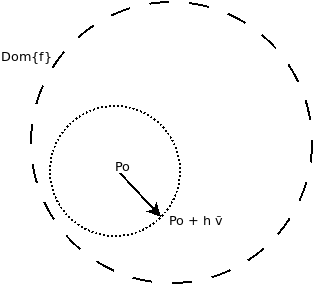
\includegraphics[scale=0.5]{img/teo_fig004_deriv_direcc.png}
\label{fig:deriv_direcc}
\end{figure}

>Entonces, se define la derivada del campo escalar $f$ en el punto $P_0$ respecto del vector $\overrightarrow{v}$ como el siguiente límite, en tanto exista:

\begin{equation}
\tcboxmath[colback=orange!25!white,colframe=orange, title=Derivada respecto de un vector]
{ f'(P_0, \overrightarrow{v}) = \lim_{h \rightarrow 0} \frac{f(P_0 + h \overrightarrow{v})-f(P_0)}{h} }
\end{equation}

Esto es una generalización que incluye a las derivadas parciales como un caso particular. Si $\overrightarrow{v}$ es un versor, la derivada es \textbf{direccional}.

Otra forma de calcular $f'(P_0, \overrightarrow{v})$ involucra una composición de funciones:

% TODO Make this work
% \includegraphics[scale=1]{img/teo_fig005_dd.png} 

Sea $g:\Bbb R \rightarrow \Bbb R / g(t) = f(P_0 + t \overrightarrow{v})$

Derivando:

\begin{equation}
g'(t) = \lim_{h \rightarrow 0} \frac{g(t+h)-g(t)}{h}
\end{equation}

Reemplazando la definición de $g(t)$:

\begin{equation}
g'(t) = \lim_{h \rightarrow 0} \frac{f(P_0 + t \overrightarrow{v} + h \overrightarrow{v}) - f(P_0 + t \overrightarrow{v})}{h}
\end{equation}

Por definición de derivada direccional:

\begin{equation}
f'(P_0 + t \overrightarrow{v}, \overrightarrow{v}) = g'(t) 
\end{equation}

Evaluando en $t = 0$:

\begin{equation}
g'(0) = f'(P_0, \overrightarrow{v})
\end{equation}

\subsection{Diferenciabilidad para campos escalares}

Sean $f$ un campo escalar, $P_0 \in \mathring{A}$, y $\overrightarrow{H} \in \Bbb R^n / (P_0 + \overrightarrow{H}) \in E(P_0, r) \subset A$. Se dice que $f$ es diferenciable en $P_0$ si y sólo si existen una transformación lineal $T_{P_0}: \Bbb R^n \rightarrow \Bbb R$ y una función $\phi_{P_0}: \Bbb R^n \rightarrow \Bbb R / \lim_{\overrightarrow{H} \rightarrow 0} \frac{\phi_{P_0}(\overrightarrow{H})}{||\overrightarrow{H}||} = 0$, que satisfagan:

\begin{equation}
\tcboxmath[colback=orange!25!white,colframe=orange, title=Diferenciabilidad para campo escalar]
{ f(P_0 + \overrightarrow{H}) = f(P_0) + T_{P_0}(\overrightarrow{H}) + \phi_{P_0}(\overrightarrow{H}) }
\end{equation}

\section{T7: Gradiente y diferenciabilidad}

Proposición: Sean $f$ un campo escalar diferenciable en $P_0$, $\overrightarrow{H} = h \overrightarrow{v}$ y $\frac{\phi(\overrightarrow{H})}{||\overrightarrow{H}||} = \psi(\overrightarrow{H})$.

Reemplazando en la definición de diferenciabilidad:

\begin{equation}
f(P_0 + h \overrightarrow{v}) = f(P_0) + \underbrace{ T_{P_0}(h \overrightarrow{v}) }_{\text{Por ser t.l., } h T_{P_0}(\overrightarrow{v})} + \underbrace{ \left|\left|\overrightarrow{H}\right|\right| }_{|h| ||\overrightarrow{v}||} \psi(\overrightarrow{H})
\end{equation}

Restando $f(P_0)$ y dividiendo por $h$ miembro a miembro:

\begin{equation}
\frac{f(P_0 + h\overrightarrow{v})-f(P_0)}{h} = T_{P_0}(\overrightarrow{v}) \pm ||\overrightarrow{v}|| \psi(h \overrightarrow{v})
\end{equation}

Tomando el límite para $h$ tendiendo a cero miembro a miembro:

\begin{equation}
\lim_{h \rightarrow 0} \frac{f(P_0 + h\overrightarrow{v})-f(P_0)}{h} = \lim_{h \rightarrow 0} T_{P_0}(\overrightarrow{v}) \pm \lim_{h \rightarrow 0} ||\overrightarrow{v}|| \psi(h \overrightarrow{v}) 
\end{equation}

Dado que por definición $\psi(\overrightarrow{H}) = \frac{\phi(\overrightarrow{H})}{||\overrightarrow{H}||}$, el segundo sumando del lado derecho tiende a cero. Y el lado izquierdo es la definición de la derivada direccional. Por lo tanto, resulta:

\begin{equation}
f'(P_0, \overrightarrow{v}) = T_{P_0}(\overrightarrow{v})
\end{equation}

Ergo, la transformación lineal de la definición de diferenciabilidad es la derivada direccional. Y además, si un campo escalar es diferenciable, existen todas las derivadas direccionales, lo cual incluye a las derivadas parciales (cuando $\overrightarrow{v}$ es un versor).

\subsection{Vector gradiente y derivada direccional}

Sea un vector genérico $\overrightarrow{H} \in \Bbb R^n$, expresado como matriz de $1xn$ o vector fila $H$:

\begin{equation}
H = \sum_{i=1}^{n} {h_i \overrightarrow{e_i}} \Rightarrow T_{P_0}(H) = \sum_{i=1}^{n}{ h_i \underbrace{T_{P_0}(\overrightarrow{e_i})}_{\text{deriv. parcial } f_{x_i}} } = \sum_{i=1}^{n}{ h_i f_{x_i}(P_0) }
\end{equation}

(Recuérdese de la sección anterior que la transformación lineal $T_{P_0}$ corresponde a la derivada direccional, y para los versores $\overrightarrow{e_i}$ eso corresponde a su vez a las derivadas parciales). La sumatoria final puede ser expresada como un producto escalar entre dos vectores de $\Bbb R^n$:

\begin{align}
    \sum_{i=1}^{n}{ f_{x_i}(P_0) h_i } &= \underbrace{ (f_{x_1}(P_0), f_{x_2}(P_0), \cdots, f_{x_n}(P_0)) }_{ \nabla{f(P_0)} = (\overrightarrow{\nabla{f}}(P_0))^T }
    \begin{pmatrix}
           h_1 \\
           h_2 \\
           \vdots \\
           h_n
    \end{pmatrix}
\end{align}

Entonces, designando a $\overrightarrow{\nabla{f}}(P_0)$ como el vector gradiente evaluado en el punto $P_0$, resulta:

\begin{equation}
T_{P_0}(H) = \underbrace{ \nabla{f}(P_0) H }_{\text{PROD. MATRICIAL}} = \underbrace{ \overrightarrow{\nabla{f}}(P_0) \overrightarrow{H} }_{PROD. ESCALAR}
\end{equation}

\begin{equation}
\tcboxmath[colback=orange!25!white,colframe=orange, title=Gradiente y diferenciabilidad]
{ \text{f es diferenciable} \Leftrightarrow f(P_0 + h) = f(P_0) + \nabla{f}(P_0) H + \phi_{P_0}(H) }
\end{equation}

Despejando $\phi_{P_0}(H)$, dividiendo por $||H||$, tomando norma y exigiendo que el límite del cociente sea cero, resulta:

\begin{equation}
\tcboxmath[colback=orange!25!white,colframe=orange, title=Gradiente y diferenciabilidad]
{ \text{f es diferenciable} \Leftrightarrow \lim_{H \rightarrow \overrightarrow{0}}\frac{ |f(P_0 + h) - f(P_0) - \nabla{f}(P_0) H| }{||H||} = 0 }
\end{equation}

Nótese que la derivada direccional es la proyección del vector gradiente sobre $\overrightarrow{v}$:

\begin{equation}
f'(P_0, \overrightarrow{v}) = \overrightarrow{ \nabla{f} }(P_0) \overrightarrow{v}
\end{equation}

Expresando este producto escalar en función de las normas y el ángulo entre ambos vectores $alpha$:

\begin{equation}
\overrightarrow{ \nabla{f} }(P_0) \overrightarrow{v} = ||\overrightarrow{ \nabla{f} }(P_0)|| cos \alpha
\end{equation}

De este modo, la derivada direccional máxima se obtiene cuando $\overrightarrow{v}$ coincide en dirección y sentido con el vector gradiente. Y en ese caso, dicho valor máximo será la norma del vector gradiente. En cuanto al valor mínimo, corresponderá a $\alpha=pi$, y será el opuesto al máximo. Por otro lado, si la derivada direccional es nula, siempre lo será en una dirección perpendicular al gradiente. Ergo, el gradiente en $P_0$ es perpendicular al conjunto de nivel 1 que pasa por $P_0$.

\begin{equation}
f \in C^1 \Rightarrow \text{f es diferenciable} \Rightarrow \left\{
\begin{array}{ll}
\exists \text{ todas las derivadas direccionales} \\
\text{f es continua} \\
\text{Todas las derivadas primeras de f son continuas}
\end{array}
\right.
\end{equation}

Ninguno de los recíprocos es verdadero. Sin embargo, este resultado es útil para aplicar modus tollens. Por ejemplo, si $f$ no es continua, no es diferenciable.

\section{T8 - Derivadas}

\subsection{Interpretación gráfica}

Sea $f$ un campo escalar en $\Bbb R^3$, diferenciable en el punto $P_0$. Por los resultados ya vistos en cuanto a diferenciabilidad, debe cumplirse que:

\begin{equation}
f(P_0 + H) = f(P_0) + \overrightarrow{\nabla{f}}(P_0) H + \theta(H)
\end{equation}

Una posible interpretación gráfica de la derivada sería:

\begin{figure}[h]
\caption{Interpretación gráfica de la derivada}
\centering
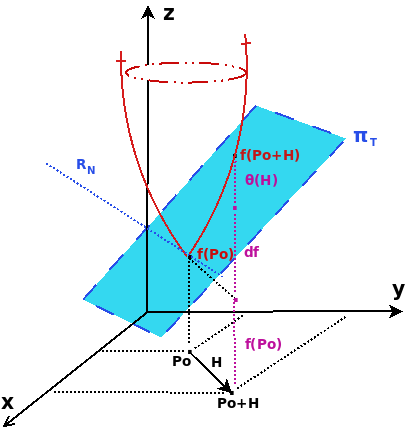
\includegraphics[scale=0.6]{img/teo_fig006_dg.png} 
\label{fig:deriv_graf}
\end{figure}

En lugar de una recta tangente, hay un plano tangente $\Pi_T$ (marcado con color cian en la figura~\ref{fig:deriv_graf}). Dicho plano es geométricamente tangente a la superficie del campo escalar en el punto $P_0$. Una forma directa de determinar el plano tangente es hallar una recta normal $R_N$, que sea ortogonal a la superficie del campo escalar en $P_0$. Dicha recta será la normal que defina el plano tangente en dicho punto.

Observando los segmentos de color fucsia, se observa que $df$ es la distancia entre $f(P_0)$ y el plano tangente. Esto se corresponde al caso de 1 variable, donde $df$ era la distancia entre $f(x_0)$ y la recta tangente. Esto permite hacer una simple extrapolación/aproximación del campo escalar $f$: $f(P_0 + H) \approx f(P_0) + df$. 

Para calcular la expresión del campo tangente, considérese:

\begin{equation}
\Pi_T: z = f(P_0) + \overrightarrow{\nabla{f}}(P_0) H + \theta(H), \text{ siendo } H = (\Delta x, \Delta y) = (x-x_0, y-y_0)
\end{equation}

De forma equivalente:

\begin{gather}
\Pi_T: z-z_0 - f_x(P_0) (x-x_0) - f_y (y-y_0) = 0 \\
R_N = N t + (x_0, y_0, z_0), \text{ siendo } N = (-f_x(P_0), -f_y(P_0), 1)
\end{gather}

Una forma más sencilla:

\begin{equation}
z = f(x,y) \Rightarrow F(x,y,z) \equiv z - f(x,y)
\end{equation}

Siendo el gradiente perpendicular al conjunto de nivel cero, o sea $\nabla{f} \perp (\text{Graf} = C_0(F))$, resulta:

\begin{equation}
\Pi_T: \nabla{F} (P - P_0) = 0, { con } P = (x,y,z)
\end{equation}

\subsection{Derivación de campos vectoriales}

\textbf{Matriz jacobiana de f}: Un campo vectorial $\overline{f}: \Bbb R^n \rightarrow \Bbb R^m$ es diferenciable si:

\begin{gather}
\overline{f}(P_0 + H) = \overline{f}(P_0) + J_f(P_0) H + \theta(H) \\
J_f(P_0) \in \Bbb R^{n x m} / J_{ij} = \frac{\partial f_i}{\partial x_j} 
\end{gather}

La matriz jacobiana $J_f$ puede pensarse como la forma más general de representar una derivada. Cubre el caso de los campos escalares (m = 1) y el caso de 1 variable (n = 1, m = 1).

\section{T9: Derivada de la composición (regla de la cadena)}

Sean $f:\Bbb R^q \rightarrow R^m$ y $g:\Bbb R^n \rightarrow \Bbb R^q$ diferenciables, y en particular sea $f$ diferenciable en el punto $g(x)$. Considérese la función compuesta $h = f \circ g = f(g(x))$. Visualmente:

\begin{figure}[h]
\caption{Composición de funciones}
\centering
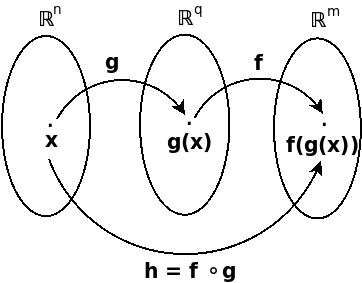
\includegraphics[scale=0.6]{img/teo_fig007_rc.png} 
\label{fig:composic_func}
\end{figure}

La regla de la cadena generalizada establece entonces que:

\begin{gather}
    \tcbhighmath[colframe=orange]{\begin{gathered}\label{equationAB}
      f:\Bbb R^q \rightarrow \Bbb R^m \wedge g:\Bbb R^n \rightarrow \Bbb R^q \text{ son diferenciables }\\
      \Downarrow \\
      h:\Bbb R^n \rightarrow \Bbb R^m / h(x) = f(g(x)) \text{ es diferenciable, y } J_{f \circ g}(x) = J_f(g(x)) J_g (x)
    \end{gathered}}
\end{gather}

Tanto en la composición como en el producto matricial, el orden es relevante.

\subsection{Derivada respecto a una recta}

Esto puede pensarse como una extensión del concepto de derivada direccional, y también como un caso particular de composición de funciones. Sea $f:\Bbb R^n \rightarrow \Bbb R$ diferenciable en el punto $P_0$, y sea la recta parametrizada $\overline{g}(t) = P_0 + t \overrightarrow{v}$, con $\overrightarrow{v} \in \Bbb R^n$. Dicha recta pasa por el punto $P_0$ y tiene su dirección determinada por $\overrightarrow{v}$.

Considérese $h = f \circ g$. Dado que $g:\Bbb R \rightarrow \Bbb R^n$ y $f:\Bbb R^n \rightarrow \Bbb R$, $h:\Bbb R \rightarrow \Bbb R$. Aplicando la regla de la cadena y evaluando en $t=0$, se obtiene un resultado conocido:

\begin{gather}
h'(t) = \overrightarrow{\nabla{f}}(g(t))  \\
h'(0) = \underbrace{ \overrightarrow{\nabla{f}}(P_0) }_{f'(g(0)) = f'(P_0)} \cdot \underbrace{ \overrightarrow{v} }_{ \overrightarrow{g}' }
\end{gather}

En palabras, $h'(0)$ es la derivada direccional de $f$ en el punto $P_0$ y la dirección de $\overrightarrow{v}$.

\subsection{Derivada respecto a una función}

Ya que se puede derivar respecto a una recta, derivar respecto a cualquier otro tipo de función no es otra cosa que derivar una composición de funciones. Por ejemplo, sea $f(x,y) = x^2 y$, que se desea derivar respecto a $y = x^2$. Pensando en términos de una composición:

Pasada a forma paramétrica, la curva $y = x^2$ resulta $\overline{g}(t) = (t, t^2)$. Esto es necesario para que las dimensiones de los dominios e imágenes concuerden y la composición tenga sentido:

\begin{equation}
\left.
\begin{array}{ll}
f:\Bbb R^2 \rightarrow \Bbb R / f(x,y) = x^2 y \\
\overline{g}: \Bbb R \rightarrow \Bbb R^2 / g(t) = (t, t^2)
\end{array}
\right\} \Rightarrow h = f \circ \overline{g} \Rightarrow h'(t) = \underbrace{ \left( \begin{matrix}2t^3 & t^2\end{matrix} \right) }_{J_f(\overline{g}(t))} \underbrace{ \left( \begin{matrix}1 & 2t\end{matrix} \right)^T }_{J_{\overline{g}}(t)} = 4t^3
\end{equation}

\subsection{Derivando por los ``caminitos''}

Esto es un abuso de notación para facilitar el cálculo de derivadas al usar la regla de la cadena.
Sean:

\begin{gather}
f: \Bbb R^3 \rightarrow \Bbb R / f(x, y, z)
g: \Bbb R^2 \rightarrow \Bbb R^3 / \overline{g}(u, v)
h: \Bbb R^2 \rightarrow \Bbb R / h = f \circ g = h(u, v) = f(g(u,v))
\end{gather}

Considérese la derivada de $h$; por la regla de la cadena:

\begin{equation}
h' = J_h = J_f(g) J_g \Rightarrow (h_u h_v) = (f_x f_y f_z) 
\begin{bmatrix}
x_u & x_v \\
y_u & y_v \\
z_u & z_v \\
\end{bmatrix}
\end{equation}

Es en este punto donde se realiza el abuso de notación; se utilizan subíndices y el producto matricial para expresar el orden de derivación a aplicar:

\begin{gather}
h_u = f_x x_u + f_y y_u + f_z z_u = \frac{\partial f}{\partial x} \frac{\partial x}{\partial u} + \frac{\partial f}{\partial y} \frac{\partial y}{\partial u} + \frac{\partial f}{\partial z} \frac{\partial z}{\partial u} \\
h_v = f_x x_v + f_y y_v + f_z z_v = \frac{\partial f}{\partial x} \frac{\partial x}{\partial v} + \frac{\partial f}{\partial y} \frac{\partial y}{\partial v} + \frac{\partial f}{\partial z} \frac{\partial z}{\partial v}
\end{gather}

Los ``caminitos'' que esto representa, visualmente, son:

\begin{figure}[h]
\caption{Regla de la cadena visualmente}
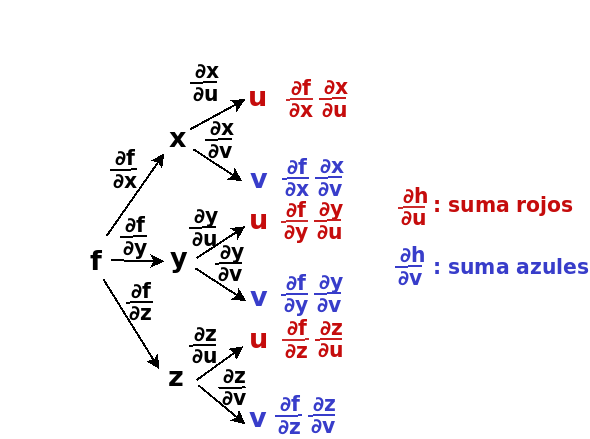
\includegraphics[scale=.5]{img/teo_fig008_rc2.png} 
\centering
\label{fig:rc2}
\end{figure}

\section{T10 - Composición II \& TFI}

\subsection{Composición}

Considérese el siguiente ejemplo de una variable:

\begin{equation}
\left.
\begin{array}{ll}
f(x) = 2x \\
f'(x) = 2
\end{array}
\wedge
\begin{array}{ll}
g(x) = x^2 \\
g'(x) = 2x
\end{array}
\wedge
h = f \circ g
\right\} \Rightarrow
\begin{array}{ll}
h(x) = 4x^2 \\
h'(x) = 8x
\end{array}
\end{equation}

La derivada puede conceptualizarse como el coeficiente de dilatación aplicado a los elementos del dominio (tomando módulo).
Por ejemplo, para $f(x) = 2x$, un intervalo de ancho $a$ en el eje x es mapeado a un intervalo de ancho $2a$ en el eje y; siendo la derivada $f'(x)=2$, esto es trivial. Para el caso más general de las jacobianas, el factor de dilatación está dado por los \textbf{determinantes jacobianos}. Por ejemplo:

\begin{gather}
\overline{f}:\Bbb R^2 \rightarrow \Bbb R^2 / \overline{f}(u,v) = (x(u,v), y(u,v)) \Rightarrow J_f(u,v) =
\begin{bmatrix}
\dfrac{\strut \partial x}{\strut \partial u} & \dfrac{\strut \partial x}{\strut \partial v} \\
\dfrac{\strut \partial y}{\strut \partial u} & \dfrac{\strut \partial y}{\strut \partial v}
\end{bmatrix} = \frac{\partial(x,y)}{\partial(u,v)} \\
|J_f(u,v)| = \frac{\partial x}{\partial u} \frac{\partial y}{\partial v} - \frac{\partial x}{\partial x} \frac{\partial y}{\partial u}
\end{gather}

\subsection{TFI: Teoremas de las funciones implícitas}

\subsubsection{Teorema de Euler}

Definición previa: función homogénea de grado $n$.

\begin{equation}
f:\Bbb R^n \rightarrow \Bbb R^m \text{ es homogénea de grado } k \Leftrightarrow f(\alpha x) = \alpha^k f(x) \text{ } \forall x \in \Bbb R^n
\end{equation}

Con esta definición, el teorema de Euler sobre funciones homogéneas establece que:

\begin{equation}
f:\Bbb R^n \rightarrow \Bbb R \text{ diferenciable en } \Bbb R^n \text{ y homogénea de grado n } \Rightarrow \overrightarrow{x} \cdot \overrightarrow{\nabla f} (\overrightarrow{x}) = n f(\overrightarrow{x})
\end{equation}

\subsubsection{Función implícita}

Supóngase $f:\Bbb R^3 \rightarrow \Bbb R$, definida como $f(x,y,z) = x^2 y^3 - z$. Considérese el conjunto de puntos $(x,y,z) \in \Bbb R^3 /f(x,y,z) = 0$, o en otras palabras el conjunto de nivel cero $C_0$. Una forma alternativa de pensar en este conjunto es como el gráfico de una función $z = \phi(x,y)$, con $Graf \phi = C_0$.

Para este ejemplo, por simple despeje, $z = x^2 y^3$. Pero en la mayoría de los casos tal despeje no es posible; sin embargo, eso no implica que $\phi(x,y)$ no exista. Existe un teorema que permite calcular las derivadas parciales de la función implícita sin conocer su expresión, dadas ciertas condiciones.

\end{document}